\part{Weekly conversation}
\section{2019/7/16 问题}

\begin{enumerate}
  \item 范式:将 PPTL 公式化成规范形式。\\
  $$Q~\equiv~\bigvee_{j=1}^{n_{0}}\left(Q_{ej}~\wedge~\varepsilon\right)~\vee~\bigvee_{i=1}^{n}\left(Q_{ci}~\wedge~\bigcirc~Q_{i}^{\prime}\right)$$

  $Q$,PPTL范式;$Q_p$,原子命题公式;$Q_i^{\prime}$,普通 PPTL 公式。

  \noindent那么PPTL 公式怎么转为范式的四种情况:(最后一种为转为完全范式)。
  \begin{enumerate}[(1)]
    \item PPTL 公式转 $\mathrm{N}_{\mathrm{F}}$。
    \item project 操作转 $\mathrm{N}_{\mathrm{F}}$。
    \item chop 操作转 $\mathrm{N}_{\mathrm{F}}$。
    \item $\mathrm{N}_{\mathrm{F}}$ $\rightarrow$ $C\mathrm{N}_{\mathrm{F}}$\\
    例 $\mathrm{N}_{\mathrm{F}}$ 转 $C\mathrm{N}_{\mathrm{F}}$
    $$\begin{aligned}\left(p \wedge \bigcirc P^{\prime}\right) \vee\left(q \wedge \bigcirc Q^{\prime}\right) \equiv &\left((p \wedge q) \wedge \bigcirc\left(P^{\prime} \vee Q^{\prime}\right)\right) \vee\left((p \wedge \neg q) \wedge \bigcirc P^{\prime}\right) \\ & \vee\left((\neg p \wedge q) \wedge \bigcirc Q^{\prime}\right) \vee((\neg p \wedge \neg q) \wedge \bigcirc f a l s e) \end{aligned}$$

    $$\left(p \wedge \bigcirc P^{\prime}\right) \vee\left(q \wedge \bigcirc Q^{\prime}\right)=false \wedge  \epsilon \vee \left(p \wedge \bigcirc P^{\prime}\right) \vee\left(q \wedge \bigcirc Q^{\prime}\right)$$
  \end{enumerate}
  \item 完全范式(作用:PPTL 完全范式否定简易)

  $$Q~\equiv\left(Q_{e}~\wedge~\varepsilon\right)~\vee~V_{i=1}^{n}\left(Q_{i}~\wedge~\bigcirc~Q_{i}^{\prime}\right)$$

  其中 $\vee_{i}~Q_{i}~\equiv~\text~{~true~and~}~V_{i~\neq~j}\left(Q_{i}~\wedge~Q_{j}\right)~\equiv~false$。

  \item 完全范式的否定\\
  例 $C\mathrm{N}_{\mathrm{F}}$ 的否定
  $$\begin{aligned}\neg \big(\left(p \wedge \bigcirc P^{\prime}\right) \vee\left(q \wedge \bigcirc Q^{\prime}\right)\big) \equiv \neg \Big( &\left((p \wedge q) \wedge \bigcirc\left(P^{\prime} \vee Q^{\prime}\right)\right) \vee\left((p \wedge \neg q) \wedge \bigcirc P^{\prime}\right) \\ & \vee\left((\neg p \wedge q) \wedge \bigcirc Q^{\prime}\right) \vee((\neg p \wedge \neg q) \wedge \bigcirc f a l s e)\Big)\\ \equiv &\left((p \wedge q) \wedge \bigcirc\neg\left(P^{\prime} \vee Q^{\prime}\right)\right) \vee\left((p \wedge \neg q) \wedge \bigcirc\neg P^{\prime}\right) \\ & \vee\left((\neg p \wedge q) \wedge \bigcirc \neg Q^{\prime}\right) \vee((\neg p \wedge \neg q) \wedge \bigcirc\neg f a l s e) \end{aligned}$$

  \item 范式图(重点)\\
  \textcolor{red}{PPTL 公式决策过程的可视化}

  NFG 举例:
\begin{figure}[!h]
  \centering
  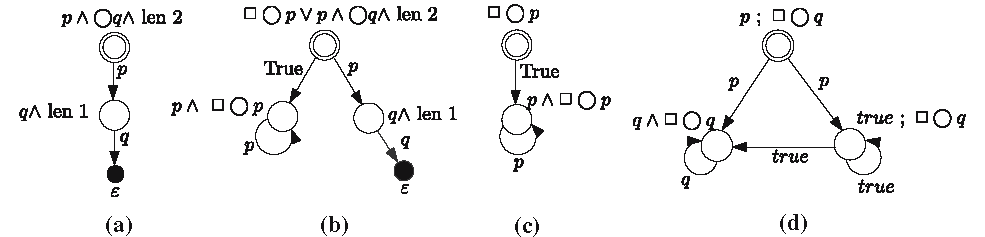
\includegraphics[width=1\textwidth]{NFG.png}
\end{figure}

  \item 带标签的范式图 \\
  由于 $prj$ 操作有明确的语义,$(P_1~,P_2)~prj~Q$ 的语义:
\begin{figure}[!h]
  \centering
  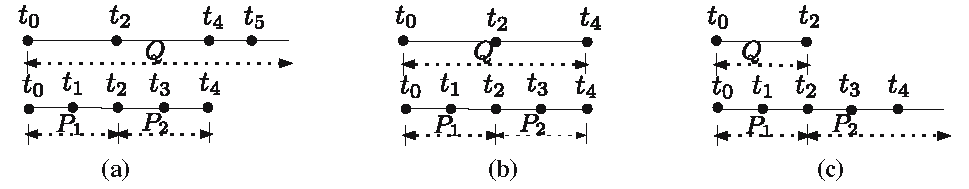
\includegraphics[width=1\textwidth]{prj.png}
\end{figure}

  即就是 PPTL 公式 $P_1$ 必须是有穷区间上的。但这一点在范式图上无法限制,所以加入标签。

\begin{figure}[!h]
  \centering
  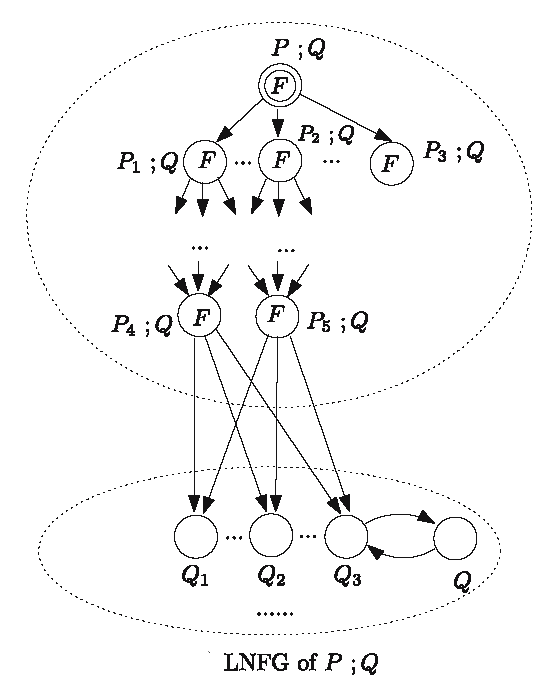
\includegraphics[width=0.6\textwidth]{LNFG.png}
\end{figure}
\end{enumerate}

\subsection{练习}

$\begin{array}{l}{\mathrm{NF}\left(\mathrm{O}^{2}(\square \bigcirc p ; q) \vee(p ; \square \bigcirc q)\right)} \\

\equiv \mathrm{NF}\left(\bigcirc^{2}(\square \bigcirc p ; q)\right) \vee \mathrm{NF}(p ; \square \bigcirc q) \\

\equiv \bigcirc(\bigcirc(\square \bigcirc p ; q)) \vee \operatorname{CHOP}(p ; \square \bigcirc q) \\

\equiv \bigcirc(\bigcirc(\square \bigcirc p ; q)) \vee \operatorname{CHOP}(\mathrm{NF}(p) ; \square \bigcirc q) \\

\equiv \bigcirc(\bigcirc(\square \bigcirc p ; q)) \vee \operatorname{CHOP}(p \wedge \varepsilon \vee p \wedge \text { Otrue; } \square \bigcirc q) \\

\equiv \bigcirc(\bigcirc(\square \bigcirc p ; q)) \vee \operatorname{CHOP}(p \wedge \varepsilon ; \square \bigcirc q) \vee \operatorname{CHOP}(p \wedge \text { Otrue; } \square \bigcirc q) \\

\equiv \bigcirc(\bigcirc(\square \bigcirc p ; q)) \vee p \wedge \operatorname{CHOP}(\varepsilon ; \square \bigcirc q) \vee p \wedge { \operatorname{CHOP}(\bigcirc true;} \square \bigcirc q ) \\

\equiv \bigcirc(\bigcirc(\square \bigcirc p ; q)) \vee p \wedge(\mathrm{NF}(\bigcirc q \wedge \varepsilon) \vee \mathrm{NF}(\bigcirc q \wedge \bigcirc \square \bigcirc q)) \vee p \wedge \bigcirc(\text {true} ; \square \bigcirc q) \\

{\equiv \bigcirc(\bigcirc(\square \bigcirc p ; q)) \vee p \wedge(f a l s e \vee \bigcirc(q \wedge \square \bigcirc q)) \vee p \wedge \bigcirc(\text {true} ; \square \bigcirc q)} \\ {\equiv \bigcirc(\bigcirc(\square \bigcirc p ; q)) \vee p \wedge \bigcirc(q \wedge \square \bigcirc q) \vee p \wedge \bigcirc(t r u e ; \square \bigcirc q)}
\end{array}$
~\\
\newpage

\section{2020/8/20 问题}
\begin{enumerate}
  \item 卷积与池化中的填充与步幅的问题。
  \begin{enumerate}
    \item tf.nn.conv2d
 \begin{table}[!h]
 \resizebox{\textwidth}{!}{
\begin{tabular}{|l|l|l|}
\hline
参数           & 内容                                                                                                                                 & 说明                                                                                        \\ \hline\hline
input        & 默认NHWC={[}batch, height, width, channels{]}                                                                                        & 默认NHWC,四维张量形式组织data\_format参数指定形式组织                                                       \\ \hline
filter       & {[}filter\_height, filter\_width, in\_channels, out\_channels{]}                                                                   & 卷积核以层定义,且同层卷积核尺寸一致。                                                                       \\ \hline
strdes       & list length 1(int),2 or 4                                                                                                          & 默认NC步幅为1;1-\textgreater{}HW;2-\textgreater{}HW;4-\textgreater{}NCHW 具体形式看data\_format组织,不支持NC维度上的步幅。\\ \hline
padding      & string-\textgreater{}'VALID' or 'SAME'; list {[}{[}0, 0{]}, {[}pad\_top, pad\_bottom{]}, {[}pad\_left, pad\_right{]},{[}0, 0{]}{]} & string:VALID-\textgreater{}不填充(舍弃);SAME-\textgreater{}输入输出等SHAPE填充,与步长也相关。list,NC维度不填充。       \\ \hline
data\_format & 默认NHWC={[}batch, height, width, channels{]}                                                                                        & CPU仿存局部性原理NHWC比NCHW更高效。但对于数据的结构,NCHW更好理解。                                                 \\ \hline
dilations    & list length 1(int),2 or 4, add 0 to input                                                                                         & 默认NC膨胀系数为1;1-\textgreater{}HW;2-\textgreater{}HW;4-\textgreater{}NCHW 具体形式看data\_format组织 \\ \hline
name         & A name for the operation                                                                                                           & optional                                                                                  \\ \hline
\end{tabular}}
\end{table}
\begin{figure}[htbp]
\centering
\begin{minipage}[t]{0.48\textwidth}
\centering
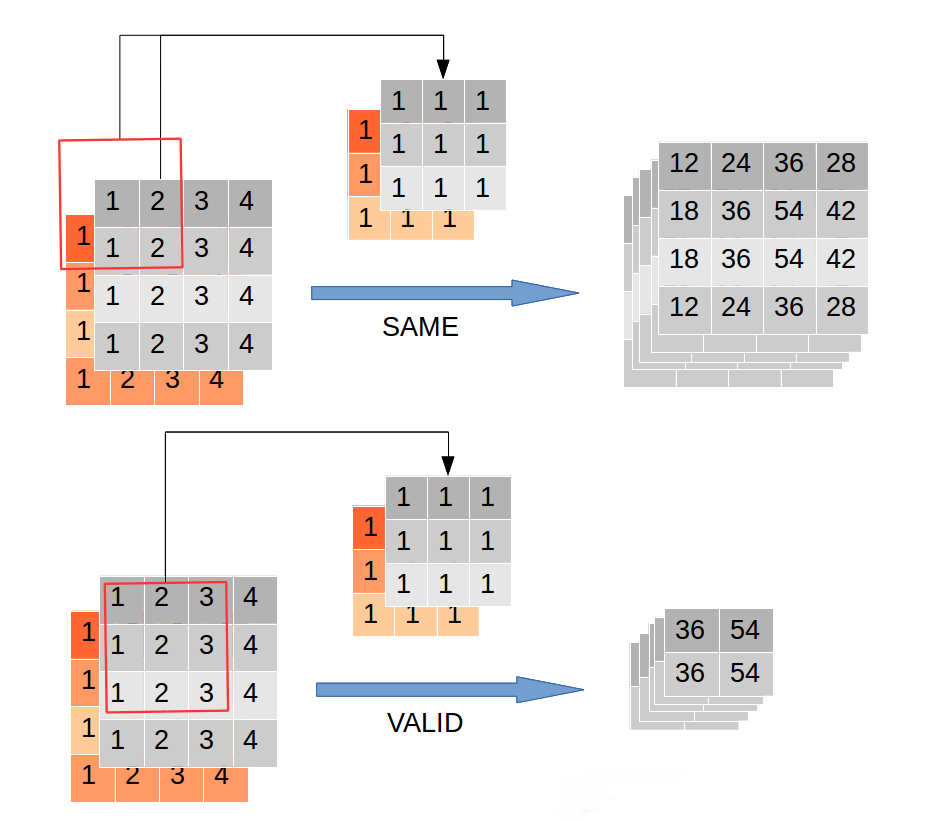
\includegraphics[width=6cm]{dilations1.png}
\caption{正常卷积}
\end{minipage}
\begin{minipage}[t]{0.48\textwidth}
\centering
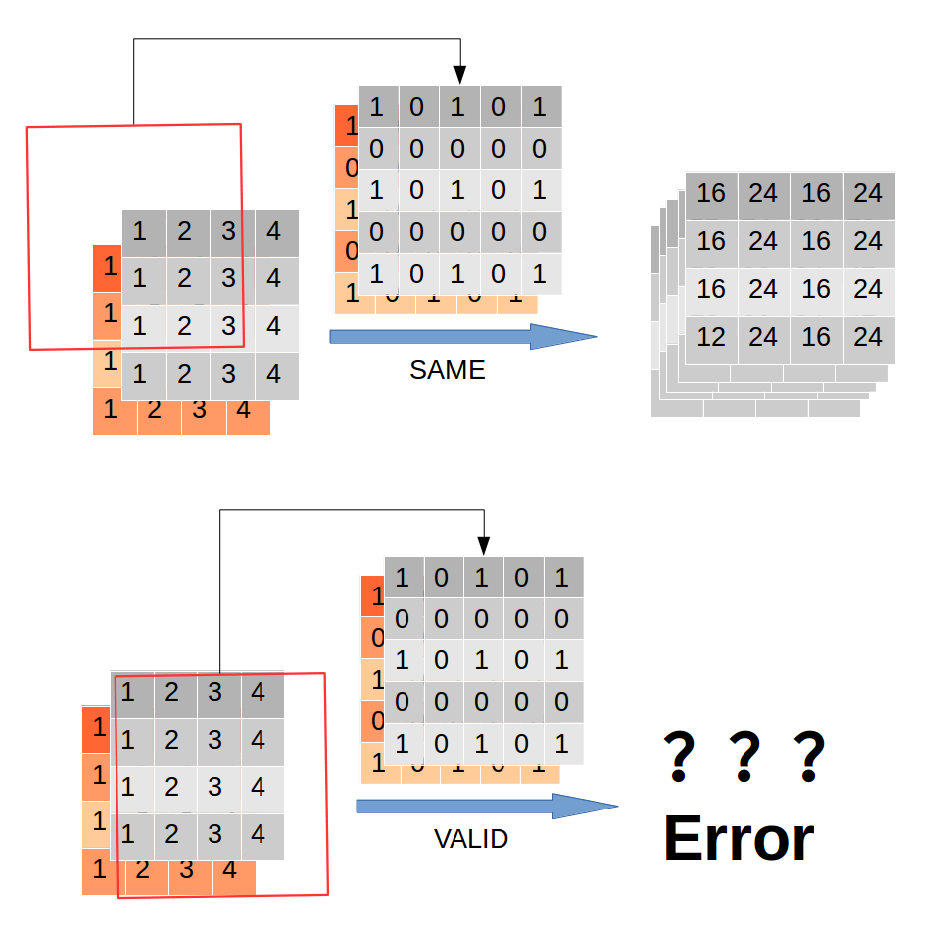
\includegraphics[width=6cm]{dilations2.png}
\caption{空洞卷积}
\end{minipage}
\end{figure}
    \item tf.nn.max\_pool
\begin{table}[!h]
 \resizebox{\textwidth}{!}{
\begin{tabular}{|l|l|l|}
\hline
参数           & 内容                                                                                                                                 & 说明                                                                                  \\ \hline
input        & 维度 N+2 N为数据单元的维度                                                                                                                   & 默认NHWC,四维张量形式组织data\_format参数指定形式组织                                                 \\ \hline
ksize        & list length 1,N,or N+2                                                                                                             & NC维度为1,其余自定义。                                                                       \\ \hline
strdes       & list length 1,N,or N+2                                                                                                             & NC维度为1,其余自定义。    不支持NC维度的步幅。                                                      \\ \hline
padding      & string-\textgreater{}'VALID' or 'SAME'; list {[}{[}0, 0{]}, {[}pad\_top, pad\_bottom{]}, {[}pad\_left, pad\_right{]},{[}0, 0{]}{]} & string:VALID-\textgreater{}不填充;SAME-\textgreater{}输入输出等SHAPE填充,与步长也相关。list,NC维度不填充。 \\ \hline
data\_format & string N==1:NWC;N==2:NHWC;N==3:NDHWC                                                                                               & 根据数据单元的维度,进行默认选取。                                                                   \\ \hline
name         & A name for the operation                                                                                                           & optional                                                                            \\ \hline
\end{tabular}}
\end{table}
  \end{enumerate}
  \noindent\textcolor{red}{注:}
\begin{itemize}
  \item  Pooling is not yet supported on the batch dimension. [Op:MaxPool]
  \item  Current implementation does not yet support strides in the batch and depth dimensions. [Op:Conv2D]
\end{itemize}
  \item 卷积核尺寸按层定义还是按网络定义。\\
  按层定义,每层的卷积核shape相同,不同的卷积核拥有不同的bias。
  \item 卷积核对应输入通道与输出通道的关系。\\
  卷积核输入通道对应input数据channel;卷积核输出通道对应output(featureMap)数据channel。
  \item 卷积神经网络一般绘图的方法。\\
  \begin{itemize}
    \item \url{http://alexlenail.me/NN-SVG/index.html}
    \item \url{https://www.zhihu.com/question/40698990}
    \item \url{https://github.com/HarisIqbal88/PlotNeuralNet}
    \item \url{https://github.com/gwding/draw_convnet}
    \item \url{https://link.zhihu.com/?target=https\%3A//github.com/ajtulloch/dnngraph}
  \end{itemize}
\end{enumerate}



\begin{lstlisting}[language=python, title=tf.nn.conv2d~~参数说明]
  '''
  conv2d_v2(input, filters, strides, padding, data_format='NHWC', dilations=None, name=None)
Computes a 2-D convolution given 4-D `input` and `filters` tensors.
Given an input tensor of shape `[batch, in_height, in_width, in_channels]`
and a filter / kernel tensor of shape
`[filter_height, filter_width, in_channels, out_channels]`, this op
performs the following:

1. Flattens the filter to a 2-D matrix with shape
   `[filter_height * filter_width * in_channels, output_channels]`.
2. Extracts image patches from the input tensor to form a *virtual*
   tensor of shape `[batch, out_height, out_width,
   filter_height * filter_width * in_channels]`.
3. For each patch, right-multiplies the filter matrix and the image patch
   vector.

In detail, with the default NHWC format,

    output[b, i, j, k] =
        sum_{di, dj, q} input[b, strides[1] * i + di, strides[2] * j + dj, q] *
                        filter[di, dj, q, k]

Must have `strides[0] = strides[3] = 1`.  For the most common case of the same
horizontal and vertices strides, `strides = [1, stride, stride, 1]`.

Args:
  input: A `Tensor`. Must be one of the following types:
    `half`, `bfloat16`, `float32`, `float64`.
    A 4-D tensor. The dimension order is interpreted according to the value
    of `data_format`, see below for details.
  filters: A `Tensor`. Must have the same type as `input`.
    A 4-D tensor of shape
    `[filter_height, filter_width, in_channels, out_channels]`
  strides: An int or list of `ints` that has length `1`, `2` or `4`.  The
    stride of the sliding window for each dimension of `input`. If a single
    value is given it is replicated in the `H` and `W` dimension. By default
    the `N` and `C` dimensions are set to 1. The dimension order is determined
    by the value of `data_format`, see below for details.
  padding: Either the `string` `"SAME"` or `"VALID"` indicating the type of
    padding algorithm to use, or a list indicating the explicit paddings at
    the start and end of each dimension. When explicit padding is used and
    data_format is `"NHWC"`, this should be in the form `[[0, 0], [pad_top,
    pad_bottom], [pad_left, pad_right], [0, 0]]`. When explicit padding used
    and data_format is `"NCHW"`, this should be in the form `[[0, 0], [0, 0],
    [pad_top, pad_bottom], [pad_left, pad_right]]`.
  data_format: An optional `string` from: `"NHWC", "NCHW"`.
    Defaults to `"NHWC"`.
    Specify the data format of the input and output data. With the
    default format "NHWC", the data is stored in the order of:
        [batch, height, width, channels].
    Alternatively, the format could be "NCHW", the data storage order of:
        [batch, channels, height, width].
  dilations: An int or list of `ints` that has length `1`, `2` or `4`,
    defaults to 1. The dilation factor for each dimension of`input`. If a
    single value is given it is replicated in the `H` and `W` dimension. By
    default the `N` and `C` dimensions are set to 1. If set to k > 1, there
    will be k-1 skipped cells between each filter element on that dimension.
    The dimension order is determined by the value of `data_format`, see above
    for details. Dilations in the batch and depth dimensions if a 4-d tensor
    must be 1.
  name: A name for the operation (optional).

Returns:
  A `Tensor`. Has the same type as `input`.
'''
  \end{lstlisting}


\begin{lstlisting}[language=python, title=tf.nn.max\_pool 参数说明]
'''
max_pool_v2(input, ksize, strides, padding, data_format=None, name=None)
    Performs the max pooling on the input.

    Args:
      input:  Tensor of rank N+2, of shape `[batch_size] + input_spatial_shape +
        [num_channels]` if `data_format` does not start with "NC" (default), or
        `[batch_size, num_channels] + input_spatial_shape` if data_format starts
        with "NC". Pooling happens over the spatial dimensions only.
      ksize: An int or list of `ints` that has length `1`, `N` or `N+2`. The size
        of the window for each dimension of the input tensor.
      strides: An int or list of `ints` that has length `1`, `N` or `N+2`. The
        stride of the sliding window for each dimension of the input tensor.
      padding: A string, either `'VALID'` or `'SAME'`. The padding algorithm. See
        the "returns" section of `tf.nn.convolution` for details.
      data_format: A string. Specifies the channel dimension. For N=1 it can be
        either "NWC" (default) or "NCW", for N=2 it can be either "NHWC" (default)
        or "NCHW" and for N=3 either "NDHWC" (default) or "NCDHW".
      name: Optional name for the operation.

    Returns:
      A `Tensor` of format specified by `data_format`.
      The max pooled output tensor.
'''
\end{lstlisting}




